\section*{Example}
Player 2 (top) took the \PPING{} action on their turn.
Because the action name is written is yellow, they played their action card face up.

\vspace{-1ex}

\begin{center}
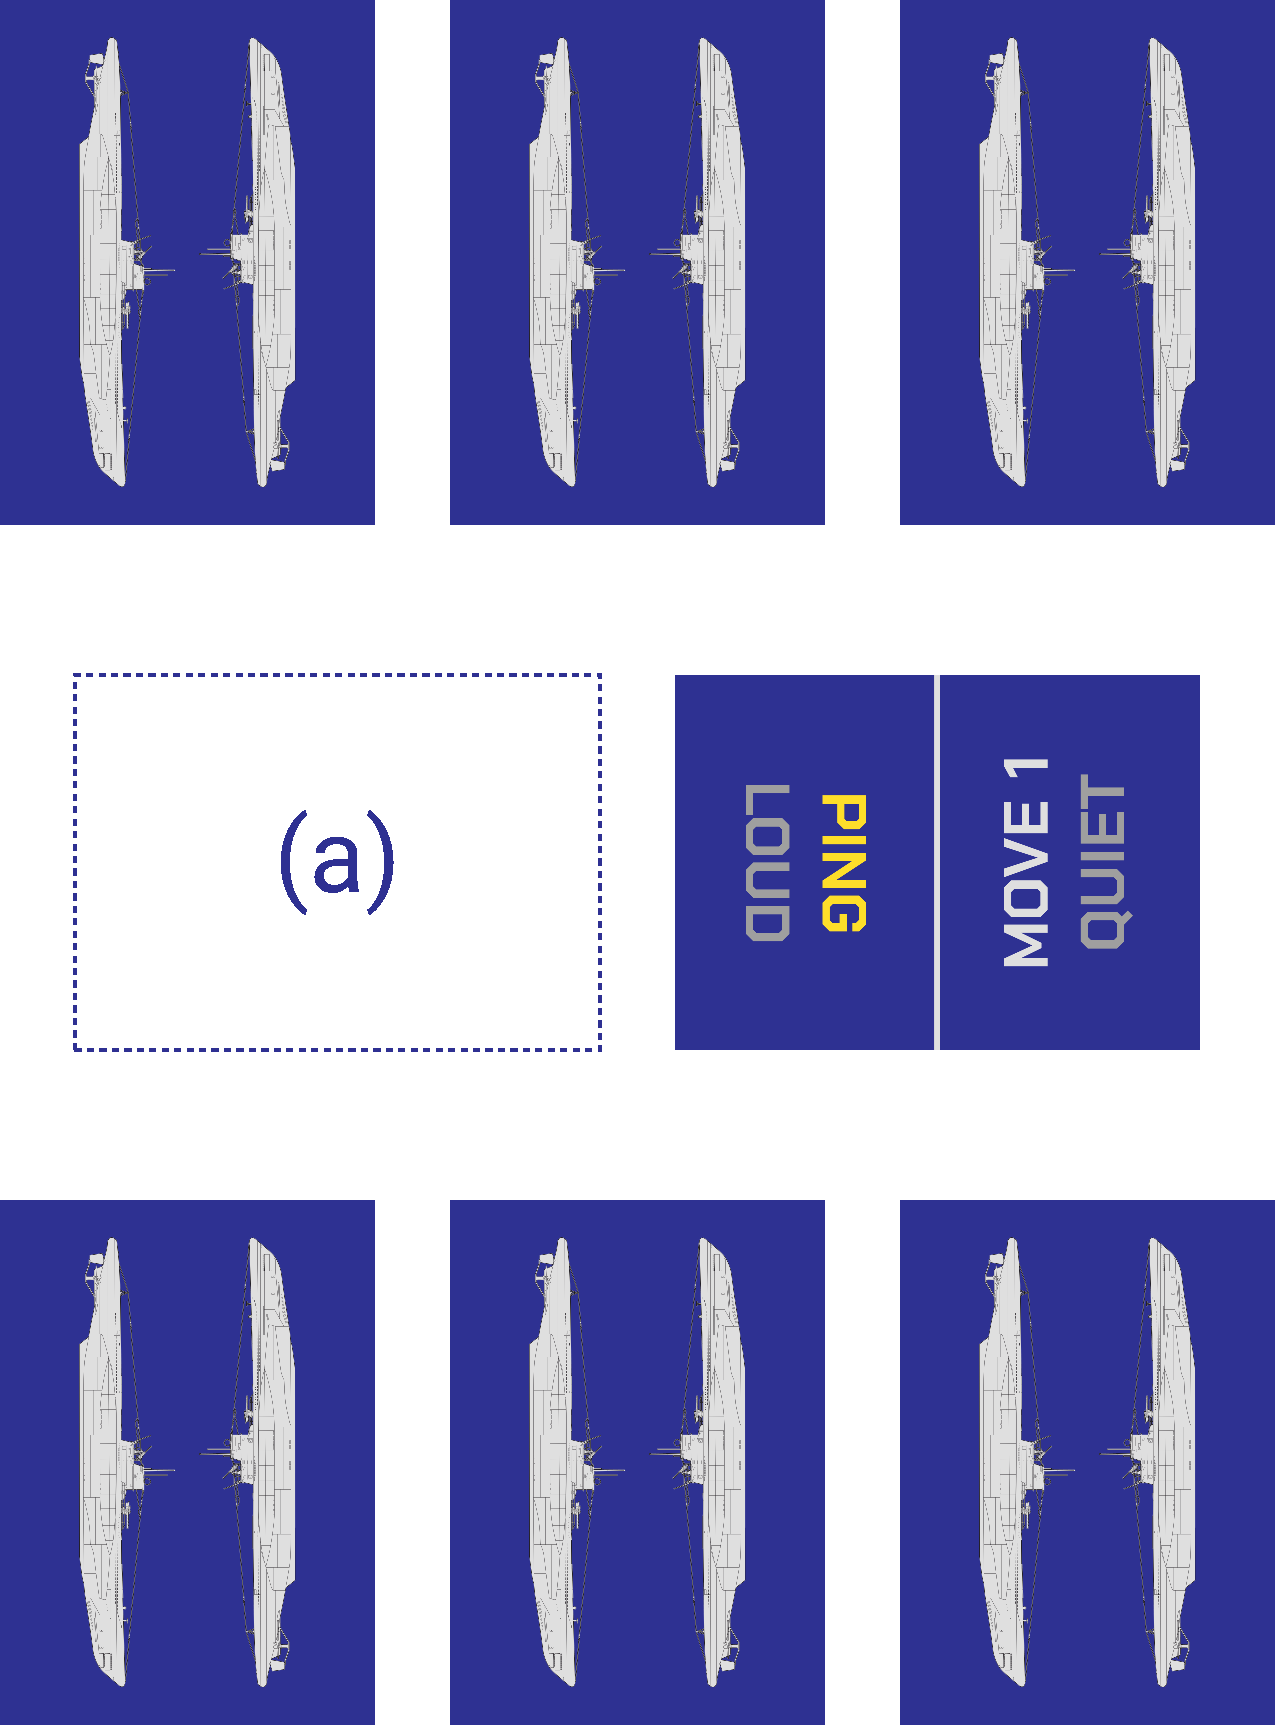
\includegraphics[width=0.5\linewidth]{example_diagram.pdf}
\end{center}

\vspace{-1ex}

Next, Player 1 (bottom) will place an action card from their hand in the play area (a).
Then, they will take the action described thereon.
Finally, they will add the action card on the right-hand side of the play area to their hand.
